%% LyX 2.1.4 created this file.  For more info, see http://www.lyx.org/.
%% Do not edit unless you really know what you are doing.
\documentclass[12pt,english]{article}
\usepackage[T1]{fontenc}
\usepackage[latin9]{inputenc}
\usepackage{float}
\usepackage{graphicx}
\usepackage[numbers]{natbib}

\makeatletter
%%%%%%%%%%%%%%%%%%%%%%%%%%%%%% User specified LaTeX commands.
\usepackage{pgfgantt}
\usepackage{adjustbox}
\usepackage{listings}
\usepackage{hyperref}
\hypersetup{pdftex,colorlinks=true,allcolors=blue}
\usepackage{hypcap}
\usepackage{a4wide}
\usepackage[hide]{ed}

\@ifundefined{showcaptionsetup}{}{%
 \PassOptionsToPackage{caption=false}{subfig}}
\usepackage{subfig}
\makeatother

\usepackage{babel}
\begin{document}

\title{MathSemantifier - a Notation-based Semantification Study}


\author{Toloaca Ion\\
Supervisor: Prof. Dr. Michael Kohlhase\\
Jacobs University Bremen}
\maketitle
\begin{abstract}
Mathematical formulae are a highly ambiguous content for which typesetting
systems as \LaTeX{} store only the rendering information. MathSemantifier
is an open-source notation-based mathematical formula semantification
system that attempts to tackle the problem of ambiguity in mathematical
documents and produce knowledge-rich equivalents. The system extracts
formulae (from formats such as \LaTeX{} or MathML) and produces content-rich
results (Content MathML) that contain no semantic ambiguity. The disambiguation
is achieved by matching the input formulae against a known database
of notation definitions, which is aggregated into a Context Free Grammar.
This paper outlines an implementation of MathSemantifier that focuses
on helping researchers in semantifying their works, and the ultimate
goal being a scalable implementation that would need minimal help
from a human, and, therefore, could be used to semantify large collections
of mathematical papers such as arXiv \citep{arXiv}.
\end{abstract}
\newpage{}

\tableofcontents{}

\newpage{}


\section{Introduction}

The scientific community produces a large number of mathematical papers
(approximately $120.000$ new papers per year), which raises the importance
of machine based processing of such documents. Unfortunately, the
most popular formats in which these papers are found (for instance,
\LaTeX{}) do not contain much information that would allow the computers
to infer the complex knowledge graph behind each paper. Since, at
this point, changing these formats is not practically possible, the
other solution is to add a semantic flavor to the existing documents
by translating them into a more suitable format, for instance, Content
MathML.


\subsection{History and Motivation}

As a system as complex as the current scientific community was created,
it went through a series of evolutions in the attempt to introduce
the best method of writing scientific documents. This process was
highly influenced by the invention and spreading of the internet.
Scientists understood the necessity of a standard that could help
them write and exchange their findings in an efficient way. A lot
of effort has gone into translating books into digital documents. 

Now, scientists have found ways to represent their knowledge in a
machine comprehensible manner, some of which are Content MathML and
OMDoc \citep{OMDOC}. These new methods do not directly store the
rendering of the documents. Instead, what is actually stored is the
knowledge graph hidden behind the ambiguity of the representation.
Naturally, these documents can be used to also generate a human readable
format, examples being Presentation MathML and \LaTeX{}.

As previously mentioned, a lot of effort went into translating books
into digital documents. Since the year of 1850, there have been produced
approximately 3.5 million papers, and approximately 120 thousand new
papers are written every year. Manual processing of such an amount
of papers in order to convert them to a semantic format is clearly
impossible. 

The next step in this evolution is translating digital documents into
improved digital documents, that the computers can actually understand
and not just store. This next step can only happen if a new, relatively
feasible, way of transition appears. As soon as the ease of transition
and the benefits from doing it outweigh the difficulties associated
with it, the scientific community will open the door into the world
where computers can actively help researchers with more than just
symbolic searches.


\subsection{Content MathML and Presentation MathML}

The two main formats \textbf{MathSemantifier }uses are Content MathML
(CMML) and Presentation MathML (PMML) \citep{W3C03}.

PMML is used to describe the layout and structure of mathematical
notations. PMML elements construct the basic kinds of symbols and
expression-building structures present in traditional mathematical
notations, containing also enough information for good renderings.
The last part is exactly the motivation as to why MathML alone is
not enough - because it only suggests specific ways of renderings,
but does not enforce stronger requirements.

CMML, on the other hand, is used to provide an explicit encoding of
the underlying mathematical meaning of mathematical expressions. This
fact is important in this context because this implies that CMML contains
no ambiguity, so, by choosing the final product to be CMML, it is
indeed possible to achieve meaningful semantification. For example,
considered ``H multiplied by e''. It can be often seen to be written
as $H$$e$ in mathematics, however, this can be interpreted also
as $H$ applied to $e$ in the context of lambda calculus, as well
as a chemical.

An example of PMML and CMML code for the expression $x+y$ is provided
in \autoref{fig:1}. Note how the \textbf{mrow} tag is used to delimit
nested expressions, while the \textbf{mo} tag indicate mathematical
objects (such as arithmetic operators) and \textbf{mi} is used for
variables and similar objects. This provides a clear structured format,
that is parsed by MathSemantifier. 

In the CMML part of the example, the \textbf{apply} tag is semantically
the application of its first element (the arithmetic plus) on two
identifiers $x$ and $y$, which altogether means simply $x+y$.

\begin{figure}[H]
\hspace{2.25cm}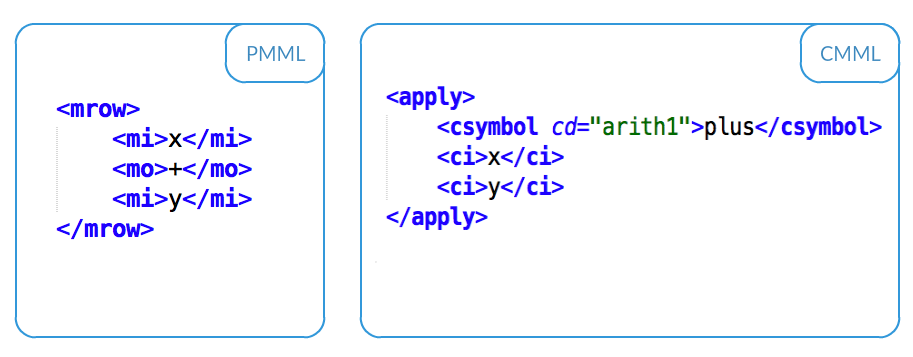
\includegraphics[width=12cm]{pmmlANDcmml}\caption{PMML and CMML \label{fig:1}}
\end{figure}


An important part of CMML is that all notations (like the arithmetic
plus notations used in the example above), contain specifications
of how these should be rendered into PMML, so the conversion is not
a problem.


\subsection{Ambiguity in Mathematical Documents}

An important concept necessary in order to understand why semantification
is a complex process is ambiguity. Mathematical documents are not
a simple collection of symbols. The main use of these documents emerges
only when the knowledge graph of a document is accessible. However,
humans tend to be lazy in writing down the whole graph, but instead
rely on implicit human knowledge to decipher these documents. This
is where ambiguity comes into play, when the author relies on the
ability of the human to use the context of document in order to pinpoint
the actual meaning an expression. Ambiguities can be largely divided
into two: structural and idiomatic ambiguities.


\subsubsection{Structural Ambiguities}

A simple example that demonstrates the concept of structural ambiguities
can be $f(a(b))$. It can mean one of the following:
\begin{enumerate}
\item Application of function $f$ to $a$ times $b$
\item Application of function $f$ to the application of $a$ to $b$
\item Multiplication of $f$, $a$ and $b$
\item Multiplication of $f$ and the application of $a$ and $b$
\end{enumerate}
Note how such a simple example with just three identifiers has at
least four different possible interpretations. It is easy to notice
that the number of readings has an exponential complexity in the length
of the expression. For instance, the expression above has $2^{n-1}$
readings, where $n$ is the number of identifiers, which is because
we can consider each application as a multiplication too.

The concept above can be generalized as structural ambiguities being
associated to different readings generated from different parse trees.
This means that the document may provide some direct clue about what
parse tree is the best, and the readings can be characterized by parse
trees.


\subsubsection{Idiomatic Ambiguities}

Contrary to structural ambiguities, idiomatic ambiguities are not
due to different parse trees. Given one single parse tree, some formulae
allow for multiple readings. A standard example would be $B_{n}$.
This could be:
\begin{enumerate}
\item The sequence of Bernoulli numbers
\item A user defined sequence
\item The vertex of one of a series of geometric objects
\end{enumerate}
In other words, the same sequence of symbols, associated with the
same parse tree can lead to multiple readings. The only feasible way
at the moment of solving such ambiguities is having a large notation
database and ultimately asking the user to choose from a list of possible
readings. \textbf{MathSemantifier} does indeed provide for the user
the complete list of possible readings, which means that it is expected
to excel at removing both structural and idiomatic ambiguities.


\subsection{Extracting Semantics from Mathematical Documents}

In this section we propose a solution to the ambiguity problem described
above. Let us recall the example from the previous section $f(a(b))$.
The first interpretation of the expression a human reader is likely
to come up with is the application of $f$ to the application of $a$
to $b$. Moreover, the other readings may take the human reader by
surprise, as he or she would assume that the first reading is the
correct one. 

Let us look into why this happens. First of all, $f$ is a symbol
humans usually use for functions, moreover, the brackets around $a(b)$
could be omitted if it were a multiplication rather than an application.
Next, $a$ and $b$ are usually used for variables, but then again
the brackets are useless if it is a multiplication. To sum up, the
human throws away meanings that would imply useless work or usage
of symbols in an unusual way. Imagine asking a mathematician which
of the expressions is more natural, $fa$ or $ab$, or, to be even
more extreme, ``Let $\epsilon>0$'' or ``Let $\epsilon<0$''.
All of these can be translated to heuristics that MathSemantifier
can use to improve its results and minimize the amount of work the
human has to do by restricting the possible meanings as much as possible.

Up until now, different heuristics used were discussed. However, mathematics
has better means of finding the one true meaning of the document.
Imagine the formula $a=b$. As a human, we can deduce it may mean
that some two objects are equal. We still have absolutely no understanding
of what those objects are, and we just assume $=$ works as a relation
on any 2 objects of the same type.

Now let us add a bit to the formula $(a=b)\wedge(b=3)$. At this point,
we deduce that $a=3$, and $=$ is a relation between numbers by applying
First Order Logic to the expression. Notice how more context reduced
the ambiguity of the previous expression. Also, notice how we naturally
assume First Order Logic is applicable to this situation. Notice also
that we are not using just heuristics, but rather we are applying
a deterministic approach to find out which meanings are impossible.

Let us consider a more interesting example $f(a+b)$. Normally, we
would assume this is a function applied to $a+b$, but nothing in
this context can help us decide against $f$ multiplied by $a+b$.
Adding an expression like $f:\mbox{R\ensuremath{\rightarrow}R}$ would
certainly help to reason against the second interpretation, because
it does not type-check.

To sum up, humans read mathematical documents bit by bit and discard
impossible interpretations until there is, hopefully, only one left.
In doing so, they mainly apply two strategies - heuristics and proof
by contradiction. This paper explores the possibility of MathSemantifier
solving ambiguities in a similar way.


\subsection{An Introduction to MathSemantifier}

In order to understand what \textbf{MathSemantifier }does, the Presentation
Algorithm needs to be explained first. The reason for that is that
\textbf{MathSemantifier }is the exact opposite of the Presentation
Algorithm, trying to convert PMML to CMML, as opposed to CMML to PMML.


\subsubsection{The Presentation Algorithm}

The presentation algorithm has its main goal to covert Content MathML
to Presentation MathML, using a database of notation renderings. In
\autoref{fig:presentation_output} a typical example of what the presentation
algorithm produces is displayed. The\textbf{ }first child of the \textbf{semantics
}node contains the PMML that corresponds to the CMML contained in
the \textbf{annotation-xml }node. In order to produce this output,
the algorithm used the notation \textbf{natarith addition (}shown
in \autoref{fig:presentation_output} as well).

\begin{figure}
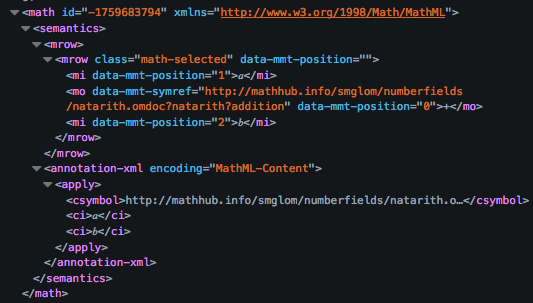
\includegraphics[bb=0bp 0bp 533bp 300bp,clip,width=8cm,height=5cm]{present_math}\hspace{0.3cm}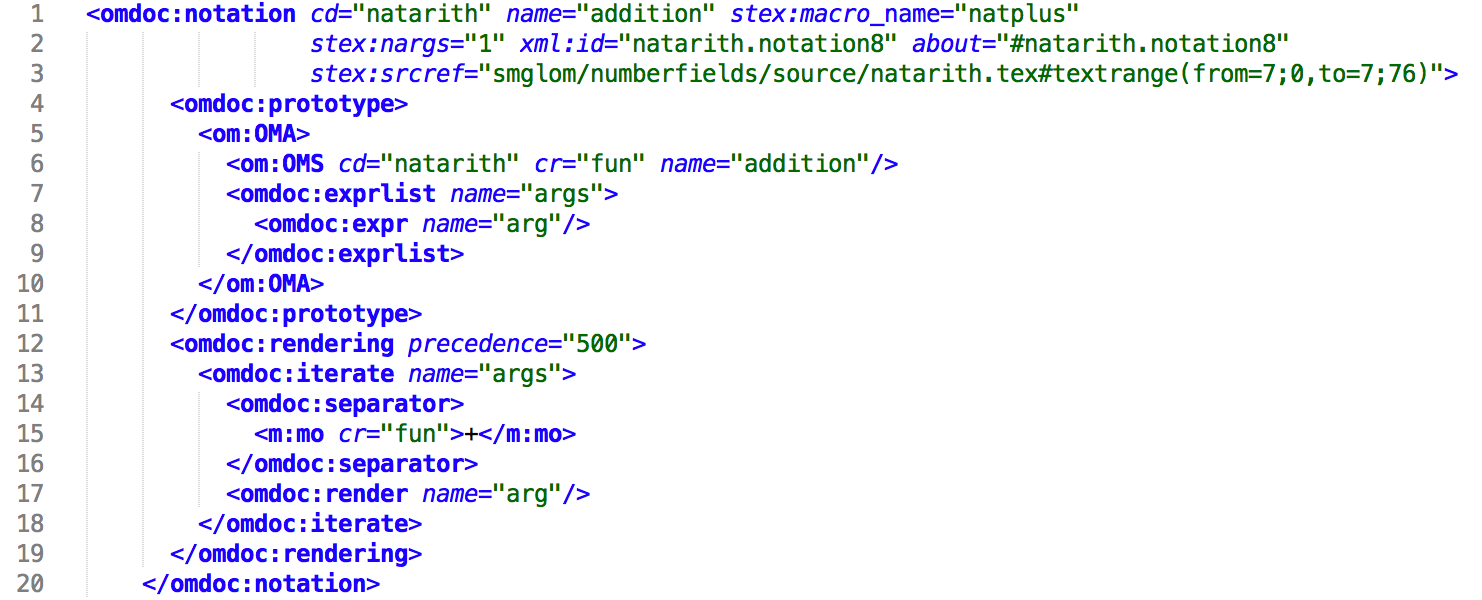
\includegraphics[width=9cm,height=5cm]{presen_not}\caption{Presentation Algorithm Output and the corresponding Notation Definition\label{fig:presentation_output}}
\end{figure}



\subsubsection{Definition of Valid Results}

The Presentation Algorithm is conceptually simple because there is
no ambiguity involved. A certain CMML expression is always presented
the same way. Even more so, the implementation is free to include
elements like \textbf{mrow }or \textbf{mspace }as long as those do
not change the meaning. However, different CMML expressions can be
rendered the same way, which is were the ambiguity of the reverse
process takes origin.

A valid result for \textbf{MathSemantifier }is, given a PMML expression,
such a CMML expression that the Presentation Algorithm can render
back to the original expression (up to \textbf{mrow }or \textbf{mspace
}tags). 

Note that, while this is certainly already a difficult task, a more
proper definition would be, given a PMML expression, a CMML expression
that can be rendered back to the original expression AND the resulting
expression represents the actual meaning of the PMML expression (or
at least, it is a valid meaning for the expression according to the
common sense of a human mathematician). \textbf{MathSemantifier }does
not explore this task beyond using some heuristics mentioned in the
further sections.


\subsubsection{Approach to Semantification}

\textbf{MathSemantifier }converts PMML into valid CMML as described
above. In order to perform this task, it needs to match PMML against
a list of notations. This is achieved by compiling the notations into
a Context Free Grammar, and using a CFG Parsing Engine to parse the
PMML. A parse returns a list of possible parse trees, out of which
\textbf{MathSemantifier }extracts information regarding what notations
matched at top level. This is then done recursively for the arguments
of the found notation. The \textbf{Implementation }section describes
in a lot more detail how the Notations are compiled into a CFG, and
how the parse trees are converted to CMML. Parsing using CFGs is a
known problem, so, instead of writing a Parsing Engine, a more reasonable
approach is using an existing one. For that purpose, the \textbf{Marpa
Grammar Engine }is used.


\subsubsection{Possible Applications of Semantification}
\begin{itemize}
\item \textbf{MathWebSearch \citep{MWS12} }(discussed in more detail in
\autoref{mws}) is a search engine for mathematical formulas. Such
search engines could greatly benefit from semantification. The idea
is that a search engine is only as good as the database of information
is. By improving the information it can search through by adding a
semantic flavor to it, a new kind of queries could be possible - semantic
queries. Rather than searching for strings, or formulas with free
form subterms, the user could specify the meaning of the sought expression.
This would improve a lot the relevance of the results, since there
will be no result that matched just because it was presented in a
similar manner. 
\item Another possibility for using semantification is theorem proving and
correctness checking. One possible application would be realtime feedback
to the user writing a paper about the correctness of the expressions
used.
\item The possibilities extend even beyond this. Using semantified content,
rather than having a database of CMML expressions, it is possible
to create a smart knowledge management system that could be used to
create expert systems. The user could then ask questions, or create
complex queries, to exploit the full power of semantic content.
\end{itemize}
Semantification will not make all of the above directly possible,
however it is a necessary step towards achieving goals similar to
the ones described above, that require more knowledge about the used
content than just how it is rendered.


\subsubsection{MathSemantifier in the Context of Disambiguation}

In the endeavor of extracting semantics from mathematical documents
MathSemantifier uses its notation database in order to attempt to
explore the space of all possible readings, and discard some irrelevant
readings using heuristics, ultimately letting the user decide which
reading is the best.

This makes clear the parts the final product excels at, but also the
main challenges related to that.

Regarding the good parts:
\begin{itemize}
\item Solving both structural and idiomatic ambiguities by exploring the
space of all readings
\item Notation addition can be easily added to the system, since the Context
Free Grammar used is generated automatically 
\item Enhanced overall user experience when writing or semantifying existing
mathematical documents by creating a dynamic, adaptive system by means
of the above mentioned strengths
\end{itemize}
The main challenges are:
\begin{itemize}
\item Scalability in the context of such a system translates into finding
the best ways to generate as few useless parse trees as possible
\item Compiling a notation database into a Context Free Grammar when including
multiple notation archives simultaneously 
\item The response time of a query to the system is a big issue, since,
as mentioned before, everything related to ambiguities has an exponential
time complexity. Finding a balance between exploring the space of
all readings enough in order to find meaningful results while keeping
the response time low is a very difficult challenge.
\end{itemize}
The rest of this paper demonstrates in detail how MathSemantifier
harnesses its strengths and solves or avoids the challenges described.


\section{State of the Art}


\subsection{Semantification}

Nowadays extracting the semantics of mathematical documents is regarded
as an interesting field, however the number of researchers in it is
limited. This is caused by several domain specific problems.

First of all, mathematics is usually represented in a format where
it mixed with natural language. Research on extracting mathematical
expressions from such contexts has not been incredibly successful
so far. Another important problem is the lack of a well prepared set
of data. This kind of data could be used for Machine Learning applications
as training data, or simply as test data for complex systems. As software
that has not been tested cannot be called particularly useful, this
poses a great problem.


\subsubsection{Restricted Natural Language}

There are multiple projects that try to use a subset of the natural
language that is still not that ambiguous but allows for intuitive
document creation. Such projects are FMathL \citep{NS10}, MathLang
\citep{KMW04}, MathNat \citep{HR10} and Naproche \citep{CKS11}.

Most such approaches try to analyze the context free parts of mathematical
expressions. We will go into more detail about Context Free Grammar
applications in semantification in the next sections. It is worthy
to note though that most such projects are not satisfied by commonly
found grammar engines, and some, like FMathL, are developing their
own specialized parsers. This paper does not outline custom parsers,
however, if further work is to be done on the subject, implementing
heuristics as to reduce the disambiguation choice list could require
at some point a similar approach.


\subsubsection{Format Conversions}

Mathematical documents in their majority are written in \TeX/\LaTeX,
but for storage and processing purposes converting them to an XML
representation is a good idea. Large scale mathematical document archives
such as $arXMLiv$ \citep{SKG} are using the \LaTeX{}ML \citep{Bru07}
converter to produce MathML and OpenMath.

\LaTeX{}ML can actually already produce Content MathML, however the
result produced in such a way from a knowledge poor setting contains
only one of the possible readings, and, therefore, is not satisfactory
from a semantic point of view as it not need satisfy the actual semantics
of the document. Enhancing \LaTeX{}ML's ability of converting \LaTeX
into knowledge rich XML format variations by exploring the space of
possible readings is one of the main goal of this thesis.


\subsection{Using Grammars for Semantification}


\subsubsection{Combinatory Categorial Grammars}

The MSc Thesis of Deyan Ginev \citep{DEYAN11} studies a similar approach
that uses Combinatory Categorial Grammars as a part of a larger analysis
pipeline that is applied to handpicked set of mathematical texts.
The results show a close to perfect recall rate with a low degree
of ambiguity. 

This approach, however, uses a manually crafted grammar as opposed
to the generated grammar used by MathSemantifier. While writing a
grammar by hand can lead to good results as mentioned above, this
approach does not scale, since it is hard to find someone who will
write such grammars every time a new notation is needed. Notations,
on the other hand, are much faster and easier to write. In other words,
scalability and extensibility are the reasons behind MathSemantifier.


\subsubsection{S-graph grammars}

The research of Alexander Koller of University of Potsdam exhibits
an interesting way of utilizing grammars for semantic construction.
S-graph grammars \citep{KOLLSG} constitute a new grammar formalism
for computing graph based semantic representations. What distinguishes
this line of research from the common data-driven systems trained
for such purposes is that S-graph grammars use graphs as semantic
representations in a way that is consistent with more classical views
on semantic construction.

S-graph grammars are introduced as a synchronous grammar formalism
that describes relations between strings and graphs, which can be
used for a graph based compositional semantic construction, which
is essentially what this paper outlines in simpler terms - using Context
Free Grammars.


\subsubsection{Marpa Grammar Engine}

As the idea of the thesis is to use a Grammar Engine, we need to introduce
a concrete solution. Text parsing using Context Free Grammars is quite
popular, and, therefore, there is quite a number of solutions, which
can, however, make the choice of the best grammar engine for a particular
purpose difficult. After comparing several such tools, the conclusion
reached was that the Marpa Grammar Engine \citep{Jeff} stands out
as a flexible, powerful and efficient tool suited for the purpose
of semantification.

To understand better the claim about efficiency, \autoref{fig:mcomp}
provides a comparison between multiple regex parsers and Marpa made
by the creator of Marpa is provided.\citep{marpaComparison}

\begin{figure}[H]


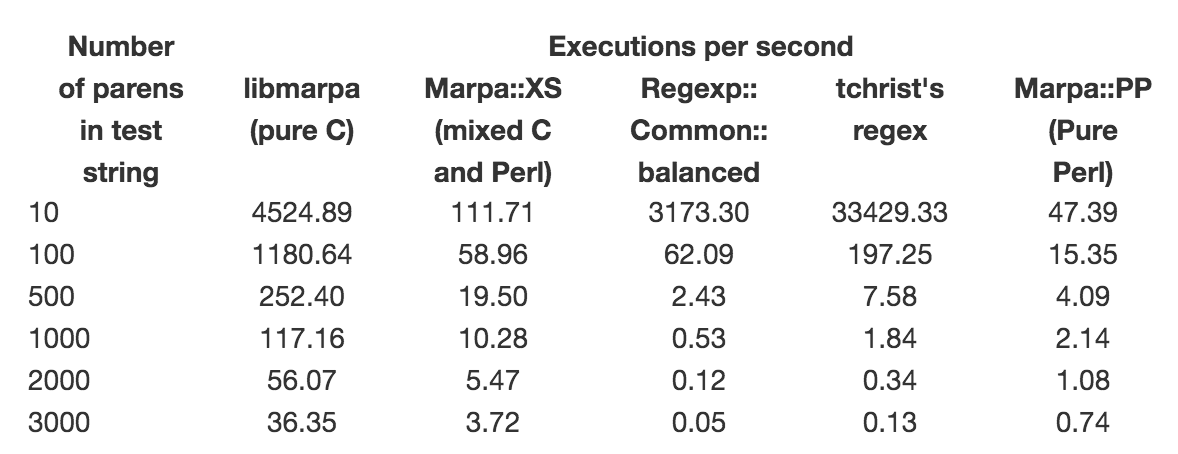
\includegraphics[width=16cm]{marpaComparison}\caption{Marpa Parser - Comparison with other Parsers \label{fig:mcomp}}


\end{figure}


The results are presented in executions per second. We can see that
standard solutions may be faster for a small nesting level, but they
go quadratic as it rises.

Another important point is that Marpa Grammar Engine has a quite simple
interface, allowing for extensive manipulations during the parsing
process. Each rules can be given an ``Action'' - a Perl routine
- that can define what the engine is supposed to do when the rules
is used. 

As it was mentioned in the previous sections, the grammar generated
is highly ambiguous, and the Marpa Engine allows for ambiguous grammar
of any kind that are required for this application.


\subsection{Extracting Formulae from Mathematical Documents \label{mws}}

As MathSemantifier as described in this paper need not be restricted
to processing just MathML formulae, but also mathematical documents
written in \LaTeX, a method of extracting MathML formulae from mathematical
documents needs to be provided. A simple way of achieving that would
be by using the same method as MathWebSearch \citep{MWS12} is using
in order to extract MathML formulae from documents containing MathML
formulae and other information. The structure of MWS is shown in \autoref{fig:mws}.
MathWebSearch accepts MwsHarvest \citep{MWSHarvest} as from the crawler
as seen in \autoref{fig:mws}. These harvests are in Presentation
MathML, therefore perfectly suited for this application.

\begin{figure}[H]
\hspace{1.5cm}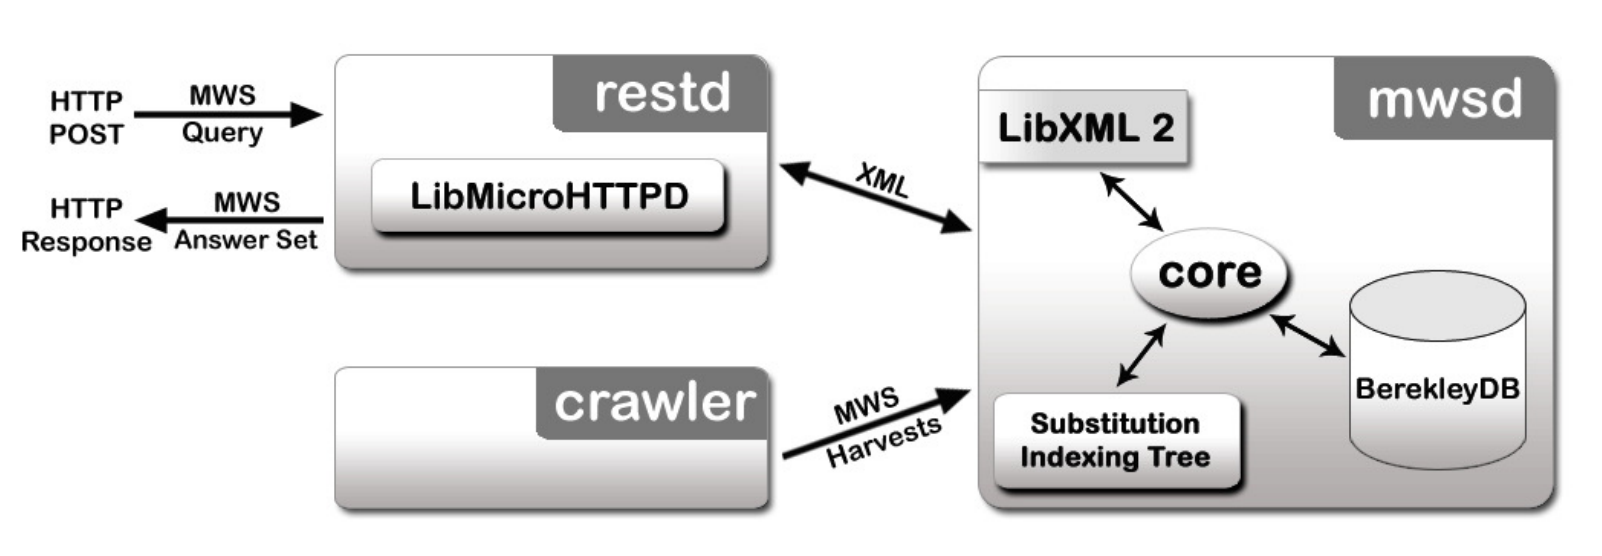
\includegraphics[width=13cm]{mwsStructure}\caption{MathWebSearch Architecture \label{fig:mws}}


\end{figure}



\section{Preliminaries}


\subsection{The Notation Database of MMT}

MathSemantifier uses a Notation Database to create the grammar it
uses. Therefore, it needs to be explained where those notations come
from. MMT \citep{MMT} (Module system for Mathematical Theories) is
a language developed as a scalable representation and interchange
language for mathematical knowledge. It permits natural representations
of the syntax and semantics of virtually all declarative languages.
The decisive factor about MMT is that there is already a large database
of notations written in s\TeX{}, which is transformed and stored in
MMT in an original format that MathSemantifier is processing in order
to generate a Context Free Grammar.

SMGloM \citep{SMGLOM} is a part of the notation database of MMT that
is especially relevant to the MathSemantifier. It contains notations
from vastly different topics of mathematics. The ones MathSemantifier
uses are number fields, algebra, calculus, geometry, graphs, magic,
sets, topology, mv, smglom, primes and numbers. SMGloM is also available
online \citep{smglomweb}.


\subsection{MMT Notation Storage Format}

The original format that MMT uses to store the notations is of high
relevance, since it the raw material from which the Context Free Grammar
is generated. The format consists of a Scala \textbf{case class }tree.
Several examples are provided in \autoref{fig:2}.

\begin{figure}[H]
\hspace{3cm}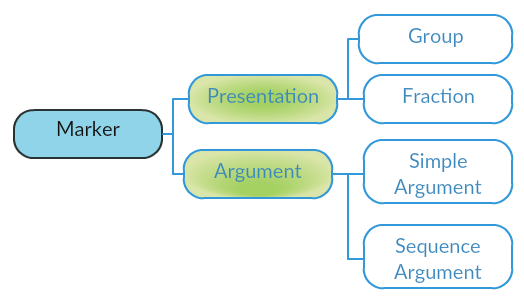
\includegraphics[width=10cm]{marker}\caption{MMT Notation Markers \label{fig:2}}
\end{figure}


Since there are about 40 types of different Markers, the tree above
is meant to simply give an idea of the structure, rather than explain
it fully. The \textbf{Marker} class is the tree of all possible notation
components. The most basic types of Markers include \textbf{Presentation
Markers }and \textbf{Argument Markers.} They have a great diversity
of subtypes. \textbf{Simple Argument }is used for single arguments,
while \textbf{Sequence Argument }is a placeholder for a sequence with
a specified delimiter. The most basic example of a sequence argument
is, if considering the example $2+3+5$, the sequence $2,3,5$ and
the delimiter $+$.

\textbf{Presentation Markers }have yet another purpose of simulating
the PMML structure. \textbf{Group Marker }stands for the \textbf{mrow
}MathML tag, \textbf{Fraction Marker }- for \textbf{mfrac }and so
on. MMT has Markers for every possible MathML tag, which goes to explain
the total number of Markers to an extent.


\subsection{\protect\LaTeX{}ML Pre-processing}

Since s\TeX{}, as an extension of \LaTeX, is just as complex to parse,
MMT uses \LaTeX{}ML in order to convert s\TeX{} to OMDoc \citep{OMDOC}.
OMDoc is then processed and stored in MMT. 

\autoref{fig:3} contains an example of the arithmetic plus notation
written in s\TeX{} and the equivalent in MathML.

\begin{figure}[H]
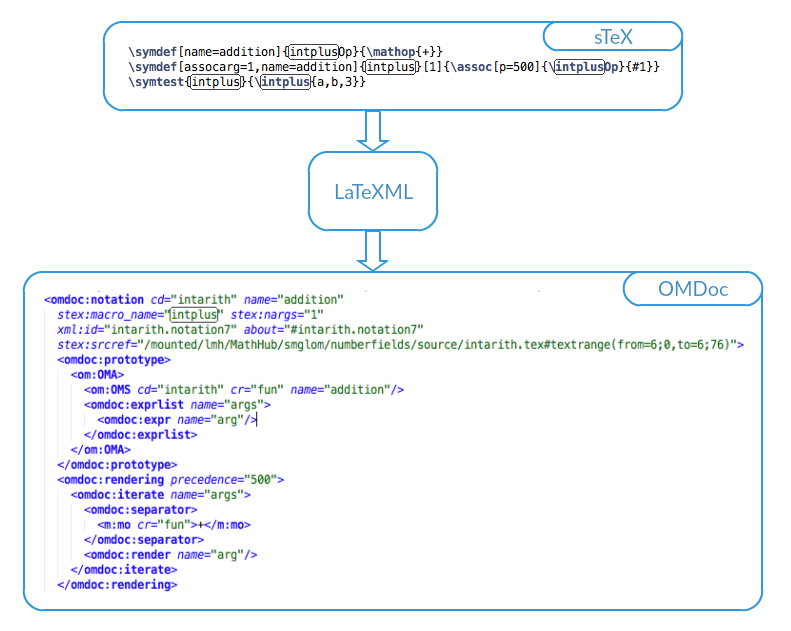
\includegraphics[width=16cm]{sTeXtoOMDOC}\caption{s\protect\TeX{} to OMDoc conversion \label{fig:3}}
\end{figure}



\subsection{Marpa Context Free Grammar Parser}

\textbf{MathSemantifier} takes the an auto-generated CFG and input
from the \textbf{Web UI} (discussed in more details in further sections)
in order to produce possible parse trees of the input. Marpa Grammar
Engine is the proposed. It was already discussed above, so let us
summarize the important points that matter for this particular application.

Marpa is \citep{marpaParser}
\begin{itemize}
\item Fast - it parses grammars in linear time. This is critical since the
size of the grammar is likely to be at least linear in the number
of notations
\item Powerful - it can parse left, right and middle recursions. Since it
is unclear what kind of recursions can occur in generated grammars,
and it would be a pity if the parse tree generator would need to be
changed midway because of it, it is better to choose something that
can handle all kinds of recursion
\item Convenient - Parser generation is unrestricted and exact, all that
needs to be provided is a CFG in BNF form. Also, if several alternatives
may yield a parse, all of them are considered. This is critical, since
this directly implies that it can deal with ambiguous grammars
\item Flexibility - it provides control over the parsing process, giving
out information about which rules have been recognized so far and
their locations. This is again extremely important because otherwise,
once again, semantification would be simply impossible
\end{itemize}
Since the CFG is ambiguous this is the most computationally intensive
part. The performance of the final product mostly depends on the efficiency
of this step.

As a side note, Marpa does not have a Scala API, so, instead, the
Perl API is used. This implies that the result parse trees need to
be transported somehow to the core application in MMT. For that purpose
LWP is used. \citep{LWP}. LWP is a set of Perl modules which provide
a simple and consistent API to the World Wide Web. After experimenting
with the API, the conclusion was that the API is simple and powerful
enough for the current purpose.


\section{The MathSemantifier System}

The major idea of \textbf{MathSemantifier }is, as already described
in the introduction, finding possible Content MathML readings for
Presentation MathML input expressions. 

The general flow of a single semantification can be described as follows:
\begin{enumerate}
\item Context Free Grammar generation from the MMT Notations 
\item Parsing using the Marpa Grammar Engine and the generated CFG to detect
the top level notation
\item Parsing the arguments of the top level notation recursively
\item Using the parse trees from step 2 and 3 to generate an internal representation
of the meaning trees
\item Converting the meaning trees to Content MathML
\item Displaying the Content MathML trees in the frontend
\end{enumerate}
The reason it was decided to use a CFG based solution is that there
exist already parsing frameworks like the Marpa Grammar Engine. It
solves all the parsing related technical problems, like parsing ambiguous
expressions, different kinds of recursion, while also providing a
high degree of freedom. 

This sections goes into the details of how exactly semantification
is accomplished. First, a general overview of the goals of the project
and its high level architecture is given. Then, each component is
described in further detail.


\subsection{Project Goals and Challenges}

The main goals of the project can be expressed in a concise manner
as follows:
\begin{enumerate}
\item Generating the correct set of parses efficiently and effectively
\item Providing opportunities for improvement for further research in the
area
\end{enumerate}
The challenges on the way of achieving a way of generating dynamically
the full set of semantic parse trees are:
\begin{enumerate}
\item Aggregating the mathematical notation database that the MMT system
into a CFG
\item Dealing with scalability issues which are entailed by ambiguity
\item The set of correct parses should be a subset of the set of generated
parses
\item The set of generated parses should ideally be a subset of the set
of correct parses too
\item Handle character encodings correctly
\end{enumerate}
This following subsections how \textbf{MathSemantifier} achieves the
above goals. 

\hyperref[6]{Section 6} shows to what extent the challenges described
are overcome and how.


\subsection{MathSemantifier \textmd{Architecture}}

The architecture can be roughly divided into four parts as shown in
\autoref{fig:7}. The components will be discussed in more details
in the further subsections.

\begin{figure}[H]
\hspace{2cm}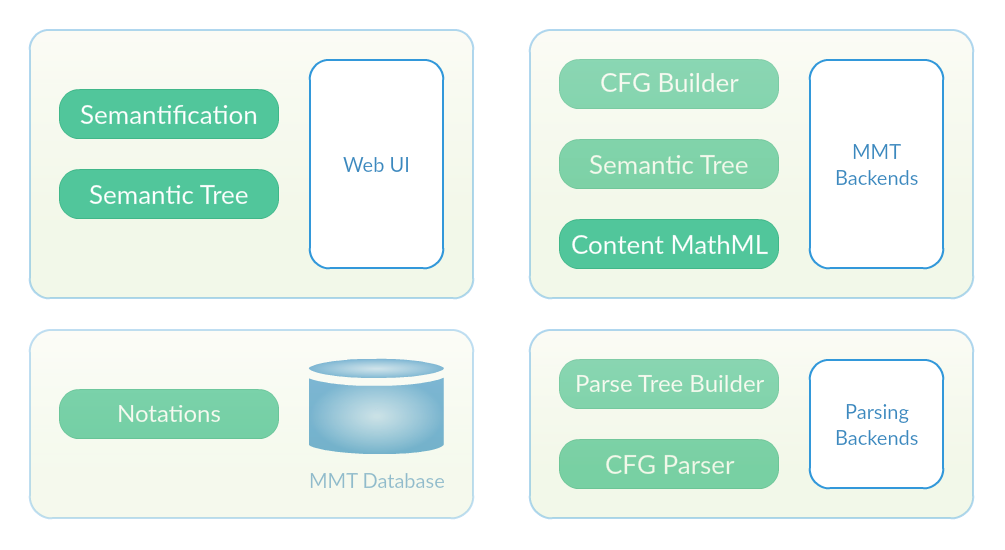
\includegraphics[width=12cm]{myThesisComponents_diagram}\caption{\textbf{MathSemantifier} Architecture \label{fig:7}}
\end{figure}



\subsection{Component communication}

Regarding the communication between parts:
\begin{itemize}
\item MMT Backends and MMT Notation DB are both part of the MMT Server Application
\item All the other connections are implemented using the \textbf{REST }protocol,
using simple \textbf{POST }requests
\end{itemize}
This also implies that the all the different components do not need
to run on one machine, especially the \textbf{Web UI }and\textbf{
}the reset of the components.

The frontend / backend separation reveals opportunities for distributed
solutions of such a system, in case scalability becomes an issue.


\subsection{Web User Interface}

The \textbf{Web UI }is a core component of \textbf{MathSemantifier.}
It is intended to be a lightweight solution that queries a server
for the results of more computationally intensive tasks.

The interface consists of an input area, where \textbf{MathML }needs
to be inputted, and three options:
\begin{enumerate}
\item Semantify (The user can guide the semantification of the top symbol
directly, by choosing the correct matching range, notation and argument
positions)
\item Show Semantic Tree (The other option is to ask for all the possibilities
and get all the semantic trees)
\item Evaluation (In this case, by repeatedly pressing this, the user is
walked through a series of examples to demo the functionality)
\end{enumerate}
The \textbf{Evaluation }option will be discussed in more detail in
\autoref{8}.

The repository containing the \textbf{Web UI }can be found on GitHub
\citep{codeWebUI}.


\subsubsection{User Guided Semantification}

The user provides Presentation MathML as input to the system, then
uses the \textbf{Semantify }button to reveal a list of top level notations
as shown in \autoref{fig:4}.

\begin{figure}[H]
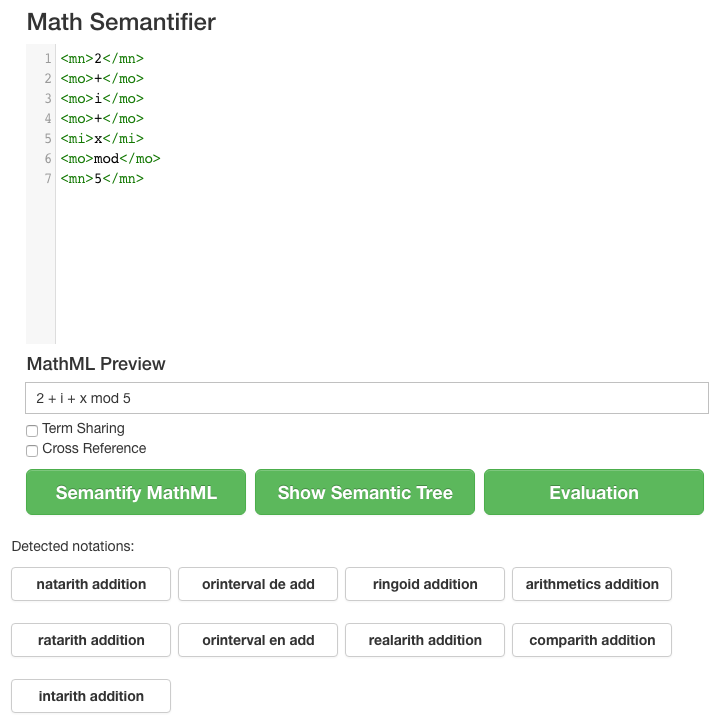
\includegraphics[width=13cm]{guided1}\caption{Top level notations \label{fig:4}}
\end{figure}


The names of the notations are derived from the notation paths as
follows: \textbf{archive name} + \textbf{symbol name.} The result
is humanly readable in most cases as seen in \autoref{fig:4}. For
example, \textbf{natarith addition }refers to the addition of natural
numbers, \textbf{comparith addition }- to the addition of complex
numbers and so on.

\begin{figure}[H]
\subfloat[Argument choice \label{fig:5a}]{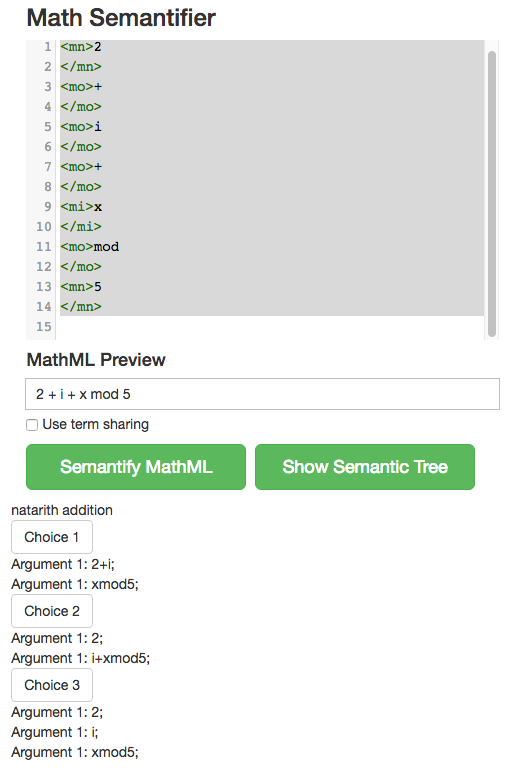
\includegraphics[width=9cm]{guided2}}\hfill{}
\subfloat[Content MathML\label{fig:5b}]{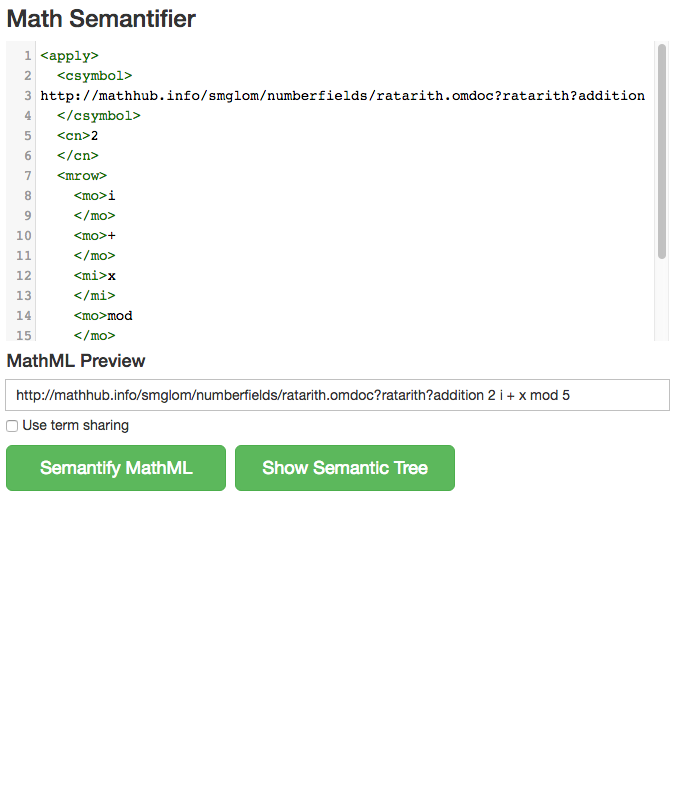
\includegraphics[width=9cm]{guided3}

}

\caption{Semantification}
\end{figure}


After determining which notation is the correct one, the user needs
to make sure that the arguments were detected properly (see \autoref{fig:5a}).

Finally, the resulting Content MathML is displayed, as shown in \autoref{fig:5b}.


\subsubsection{Semantic Tree Generation}

The easier but computationally more expensive alternative is to simply
generate all the possible parse trees at once and display them. The
user simply needs to click the \textbf{Show Semantic Tree} option.

\begin{figure}[H]
\hspace{2cm}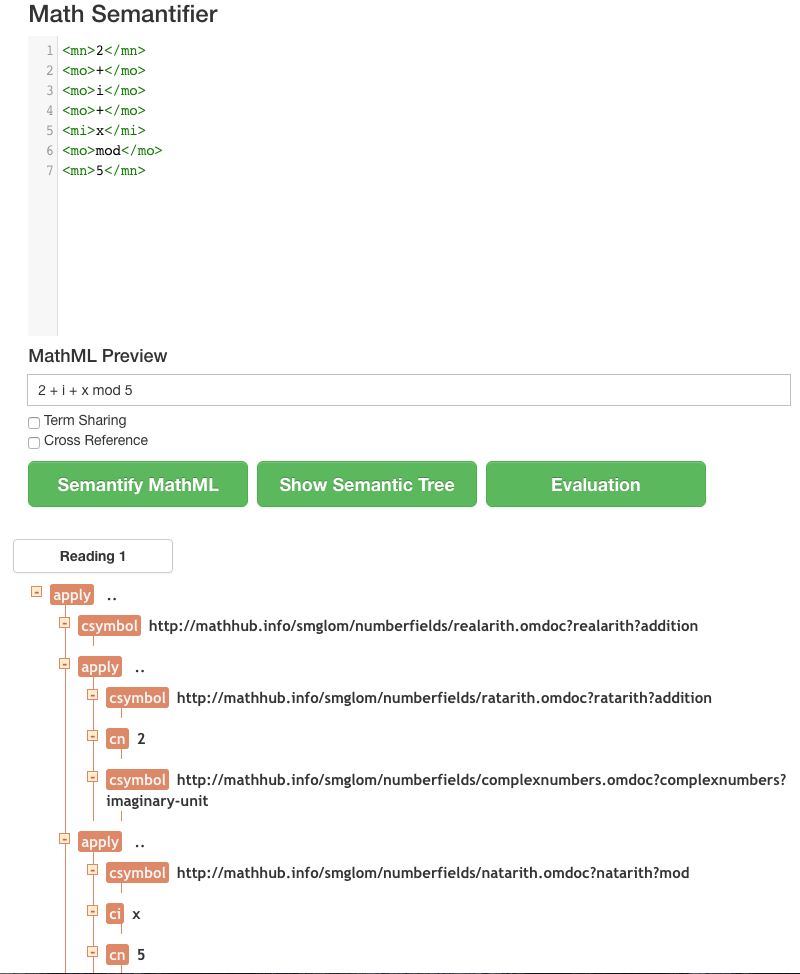
\includegraphics[bb=0bp 5bp 800bp 972bp,clip,width=12cm]{auto1}\caption{Semantic Tree Results \label{fig:6}}
\end{figure}


For the example shown in \autoref{fig:6}, there is a total of 342
different readings. This can be easily explained, since \textbf{Invisible
Times}, \textbf{Arithmetic Plus} and \textbf{Mod }have each multiple
notations definitions (that originate from different MMT archives,
for instance), and there are no limitations on what kind of notation
definitions can go together in the same CMML tree.


\subsubsection{Term Sharing}

In order to minimize the Content MathML, the standard allows subtree
sharing. To enable this option, the \textbf{Use term sharing }checkbox
should be checked. In that case, the terms is shared along different
readings. This feature could be useful for an application that requires
all the possible readings, to minimize user interaction, for instance. 

The current implementation shares the CML generated at any recursion
level. This implies that only \textbf{apply }or \textbf{csymbol }which
correspond to some part of the input can be shared. This can be improved
upon, by also sharing ground terms and other parts of the notations.
More importantly, this type of sharing is incompatible with cross-referencing,
since it may share subtrees that have common ancestors. For instance,
$1+1$ has two instances of one, however, it may not be shared, because
each instance corresponds to a different presentation element. 


\subsection{MMT Backend}

The MMT Backend is a \textbf{Server Extension }that is part of MMT.
As shown in \autoref{fig:7}, it is linked via \textbf{REST} with
the \textbf{Web UI }and the \textbf{Parsing Backends.} 

Its role can be summarized to the following core functions:
\begin{enumerate}
\item Compile the \textbf{MMT Notations} into a CFG Grammar
\item Receive the input from the \textbf{Web UI} and build its Semantic
Tree
\item Delegate the parsing to the \textbf{Parsing Backends}
\end{enumerate}
I decided to put the core logic of the application in MMT in order
to make it easier to interoperate with the MMT Notation Database,
as well as with any other MMT components that may want to need \textbf{MathSemantifier.}
By the current design, using \textbf{MathSemantifier }within MMT is
as simple as a function call that takes the input as a string.

The code can be found as part of the MMT codebase \citep{codeMMT}.

Let us look at the components of the MMT Backends in more detail below.


\subsubsection{Context Free Grammar Generator}

The Grammar Generator aggregates all the knowledge contained in the
MMT Notations into one Context Free Grammar. The grammar is shaped
into the normal form accepted by the Marpa Grammar Engine. To achieve
this, the format used to store the notations in MMT is decomposed
into CFG rules. Otherwise said, the tree-like structure of each formula,
that is stored as nested applications of \textbf{MMT Markers }(discussed
previously) needs to be serialized into CFG rules.

This is done in several steps:
\begin{enumerate}
\item Break apart the \textbf{MMT Marker }trees into level by level representations
\item Transform the intermediate representation into valid CFG rules
\item Optimize if possible (will be discussed in detail in the subsequent
sections)
\end{enumerate}
The fundamental structure of the CFG is established using a preamble
as shown in \autoref{fig:cfg_preamble}. Note the default action is
the \textbf{Grammar Entry Point.} It is precisely what tells the Grammar
Engine to build parse trees, and also determines their structure.

The entry point into the grammar is the \textbf{Expression }rule.
It can be an MMT Notation, or Presentation MathML. The \textbf{prec0}
rule should be read as precedence zero, that is - the lowest precedence
there is.

\begin{figure}[H]
\hspace{2cm}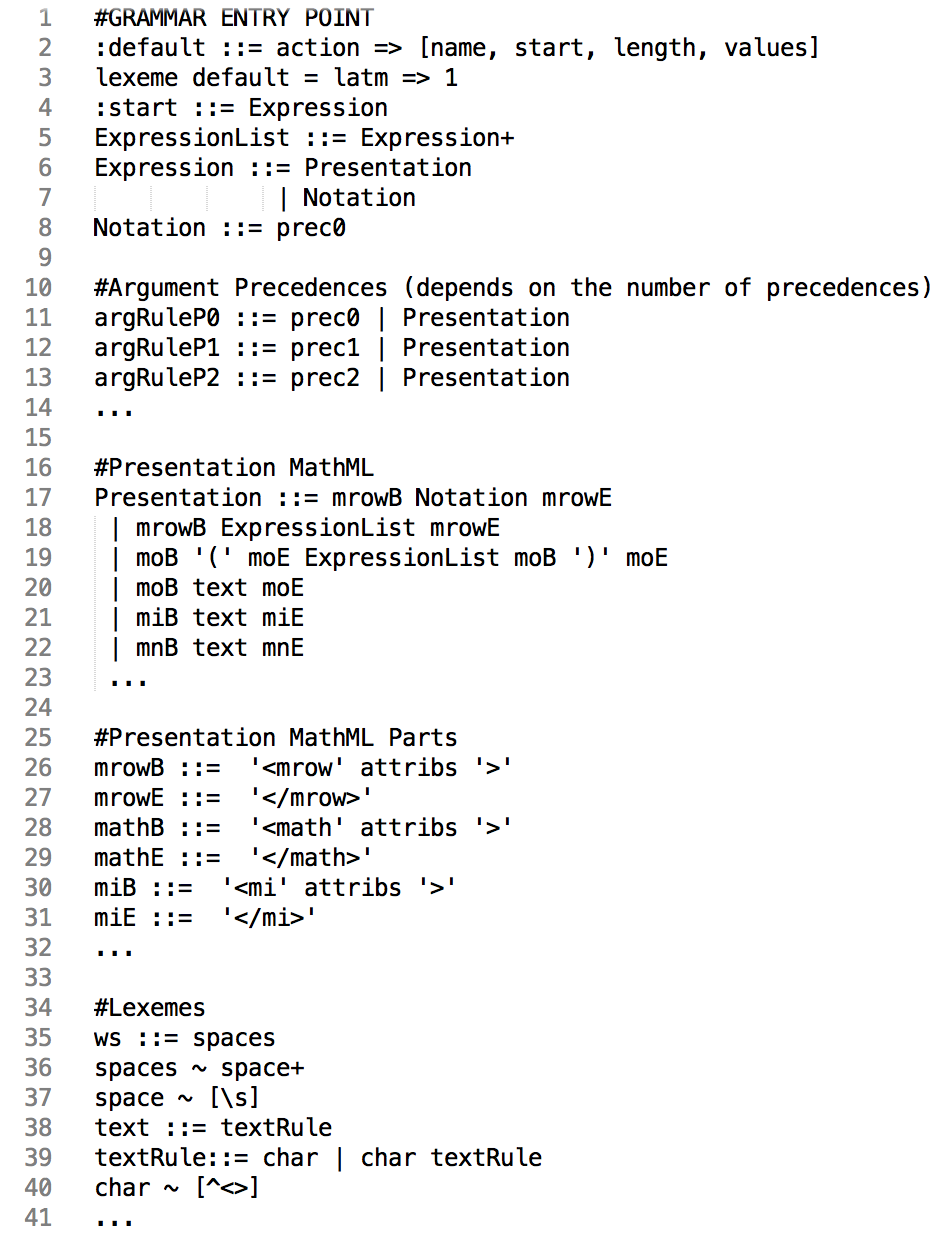
\includegraphics[width=8cm]{cfg_preamble}

\caption{CFG Preamble\label{fig:cfg_preamble}}
\end{figure}


Precedence handling is done using a commonly used method for including
it in CFGs. The \textbf{Notation Precedences }section in \autoref{fig:cfg_preamble}
gives a quick glance at how exactly it is done. The number of precedences
needs to be known in advance, then, for each precedence value a corresponding
\textbf{precN} rule is created.

The rule contains all the notations with that precedence, and, one
of the alternatives is going to a higher precedence value. In the
example below there are 15 used precedence values (\textbf{prec0 }corresponds
to precedence $-\infty$). However, the \textbf{Notation Precedences
}section shows only half of the concept.

To make this approach work, what is also needed is that the arguments
in a rule of a certain precedence N can only contain notations with
precedence $K$ if $K>N$. This is done by the \textbf{Argument Precedences
}part in the preamble (as shown in \autoref{fig:cfg_preamble}).

Finally, \autoref{fig:cfg_ex} presents an example of what the \textbf{natharith
addition }MMT notation from the \textbf{smglom/numberfields }archive
translated to CFG rules looks like.

\begin{figure}[H]
\hspace{2cm}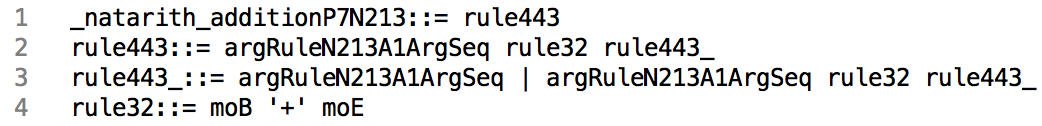
\includegraphics[width=10cm]{cfg_ex}\caption{ MMT Notation in CFG\label{fig:cfg_ex}}
\end{figure}



\subsubsection{Semantic Tree Generator}

The \textbf{Semantic Tree Generator }works by recursively querying
the \textbf{Parsing Backend }and using the result to construct a the
tree of possible meanings.

The parse trees stored in MMT have the following structure:

\begin{figure}[H]


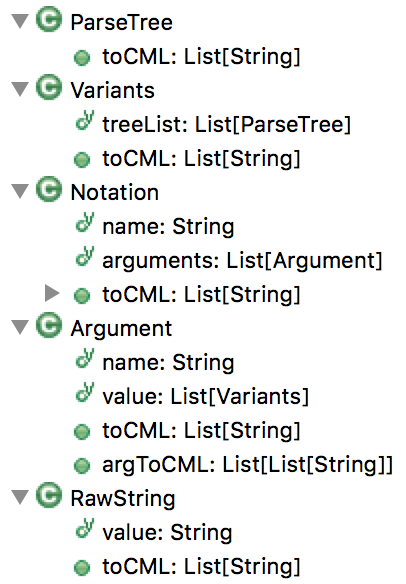
\includegraphics[scale=0.7]{parseTreeStructure}\caption{Semantic Parse Tree Structure \label{fig:8}}


\end{figure}


This simple structure shown in \autoref{fig:8} allows for a flexible
way of parse tree storage. 
\begin{itemize}
\item \textbf{Variants - }represents a list of possible readings. It is
always be the top node in any parse tree.
\item \textbf{Notation - }a notation detected in the input. It contains
its name and arguments.
\item \textbf{Argument - }an argument of a notation. The plugin is recursively
called on it to construct its meaning subtree as well.
\item \textbf{RawString - }the ground term representation
\end{itemize}
This structure is important because, in case another application wants
to access the parse trees and process them, this structure will need
to be dealt with.




\subsubsection{Content MathML Generator}

The final part of any of the semantification processes is converting
the internal representation to a standard one, which is CMML in this
case. MMT provides a simple API which requires:
\begin{enumerate}
\item The MMT notation path
\item The argument maps (maps from the argument number to the corresponding
substring)
\end{enumerate}
Both of which are available in my representation structure. The argument
path is obtained by extracting the argument number from the argument
name, and looking up in a map of paths created at the time of grammar
creation. This implies the grammar rule names are overloaded with
meaning, however, the possibilities are very limited in this aspect
since the parsing framework used does not give complete control over
the parsing process.


\subsection{Parsing Backend}

The Parsing Backend \autoref{fig:7} receives requests from the \textbf{Web
UI }directly for Guided Semantification and from the \textbf{MMT Backend
}for Semantic Tree Generation. All the parsing related work is delegated
to this backend, to the extend that it even includes the substrings
where the arguments of the notations match (I will explain in more
detail why in \autoref{encoding_issues}).

The code of the Parsing Backend can be found on GitHub \citep{codeParsingBackend}.

The parsing backend consists of two parts. 


\subsubsection{Context Free Grammar Parser}

First of all, the the CFG needs to be queried and parsed. This is
implemented using lazy evaluation, which means that it is only done
when a request actually comes.

The serialized CFG is unpacked and feed to the Marpa Parser Generator.


\subsubsection{Parse Tree Generator}

The more complex of the two parts is actually going through the parse
trees and extracting useful information. Note that going through all
the parse trees is not practical, so only the first $N$ (currently
$1000$) parse trees are processed. This still gives the correct results
in most cases since the grammar rules are optimized for giving preference
to parse trees that are more likely to be correct (discussed in more
detail in \hyperref[6]{section 6}).


\subsection{Encoding issues \label{encoding_issues}}

Since \textbf{MathSemantifier }deals with unicode, and has parts written
in Javascript, Scala and Perl, which treat unicode symbols differently,
it needed a solution for this problem. Javascript and Scala have \textbf{UTF-16
}strings, while Perl has \textbf{UTF-8 }strings. The implemented solution
simply passes around the string encoded using \textbf{encodeURIComponent
}in Javascript or its equivalents in other languages, and only the
parsing backend in Perl actually deals meaningfully with substrings.
The result of the parsing backend contains the complete substrings
for the matched rules and arguments. This also represents an opportunity
for improvement, since passing around positions in a string is more
efficient that substrings.


\section{\label{6}Optimizations and Heuristics}

This section describes the attempts made in order to deal with the
overwhelming ambiguity of mathematical notations and produce actual
results. 
\begin{enumerate}
\item Only notations on the whole input are matched. Subterms are matched
directly by the \textbf{Semantic Tree }plugin.
\item The number of parse trees is limited to $N=1000$. The number of parse
trees was empirically determined to include the set of correct parses
for the examples used (see the \textbf{Evaluation }section\textbf{).}
\item The non-empty alternatives in the CFG are put first. The Grammar Parser
has a predictable behavior of going through the alternatives left
to right, and since empty rules match \textbf{always}, it is imperative
that other alternative are attempted first. Note that only after this
optimization any kind of results were possible to achieve on non-trivial
input.
\item The CFG includes precedences correctly. This weeds out a large number
of incorrect readings.
\item Sub-term sharing is part of the \textbf{MathML }standard, and within
one request, if sub-term sharing is enabled, the response tries to
share its terms as much as possible in order to compress the output.
\item \textbf{The Semantic Tree }plugin makes use of memoization to reduce
one dimension of the exponential blowup as explained on the following
example. \textbf{$2+3$ }has 6 possible readings, because $+$ is
defined 6 times, between natural, integer, real numbers and so on.
However, $2$ and $3$ - these subterms do not contain any notations,
yet, the plugin needs to know that for every possibility of $+$.
Memoization allows to omit a large number of \textbf{POST }requests
even in this simple example, which results into a significant speedup
of a factor of approximately 4 (13 \textbf{POST} requests vs 3 \textbf{POST
}requests). Also, slight modification of the input benefit of a significant
speed-up, as well as using a previous input as a subterm in a new
input.
\end{enumerate}

\section{\label{8}Evaluation }

This section presents an evaluation of \textbf{MathSemantifier }from
the point of view of efficiency and effectiveness of semantic tree
generation. Next, the interoperability of the system with other possible
applications is examined, which mostly depends on the backend APIs.


\subsection{Semantic Tree Generation}

Testing \textbf{MathSemantifier} through normal operation is not a
trivial task, because the results need a human expert to check whether
the results are indeed correct. Fortunately, the \textbf{MathHub Glossary
\citep{glossary}} contains a sufficient number (about 3000) of examples
of Presentation MathML with Content MathML annotations that result
from applying the \textbf{Presentation Algorithm} discussed in the
introduction. Since \textbf{MathSemantifier }is the partial inverse
of the \textbf{Presentation Algorithm, }checking whether the results
are indeed correct boils down to comparing two Content MathML trees.

For the purpose of testing \textbf{MathSemantifier} on the \textbf{MathHub
Glossary, }the \textbf{Evaluation }option mentioned in the \textbf{Web
UI} section is used. It walks the user through the examples extracted
from the \textbf{MathHub Glossary. }A typical example looks as shown
in \autoref{fig:eval_ex}.

\begin{figure}[H]
\hspace{2cm}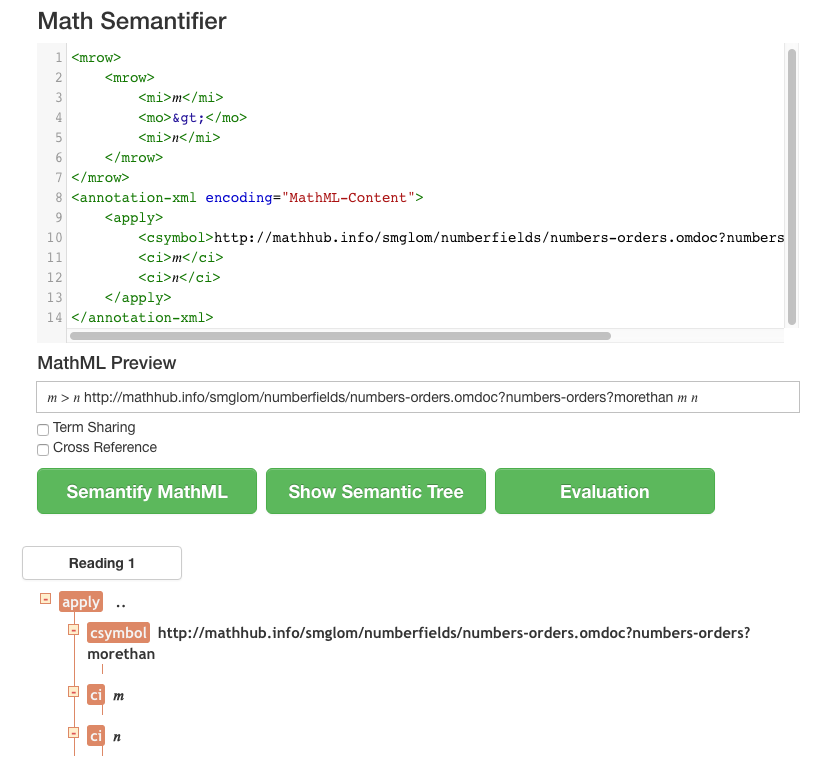
\includegraphics[width=10cm]{eval}\caption{Glossary Example \label{fig:eval_ex}}
\end{figure}


The editor displays the example itself, which contains the PMML and
the corresponding CMML it was generated from using the Presentation
algorithm. The readings are displayed below in a manner that makes
reading more efficient.


\subsubsection{Results}

A visual control revealed the following approximate results for the
testing on the \textbf{MathHub Glossary. }About 40\% of the examples
are semantified correctly. However, this is largely because of reasons
that do not depend on \textbf{MathSemantifier} itself.

Contrary to what the numerical result suggests, for expressions with
less than 1000 parse trees that are correctly rendered, \textbf{MathSemantifier
}produces correct results with a very high probability.

Let us look into the reasons that make \textbf{MathSemantifier }fail.
First of all, the reasons that do not depend on the system itself.
\begin{enumerate}
\item The Presentation Algorithm fails to render CMML into PMML properly.
This may very well be the main reason for failure. I estimate that
about 30-40\% of the \textbf{Glossary }examples are not rendered properly.
\item About 10\% of the examples include symbols from archives that were
not included when generating the CFG that \textbf{MathSemantifier
}is using. This is a limitation that could be easily overcome by adding
those symbols, but, as a proof of concept, having a complete coverage
of the symbols was not the primary focus.
\end{enumerate}
Up to this point, if we exclude the above mentioned examples, the
effective success rate of \textbf{MathSemantifier} is about 80-90\%.
\begin{enumerate}
\item Some notations are omitted (mainly because their rendering consists
only of one argument rendering, which creates cycles in the CFG).
This limitation is considerably hard to work around, since it increase
drastically the ambiguity of the input if we allow free form subterms
anywhere.
\item Too long inputs / \textbf{MathSemantifier }only considers the first
1000 parse trees as mentioned in the \textbf{Heuristics }section above.
An obvious fix would be increasing the number of considered parse
trees, however this would result into a significantly worse performance.
Even for further attempts I would recommend failing early (allowing
for 80-90\% of requests to complete on average) and retrying again
with other parameters rather than waiting for too long. In any case,
using a huge auto-generated CFG is certainly a big limitation for
the performance.
\item \textbf{MathSemantifier} assumes that the input has only one top level
\textbf{mrow} or a single bracketed list of expressions. This technical
limitation is still present because the number of notations that actually
do that is quite low as seen in practice, however it is not impossible
to fix, even in the current setup.
\item One last interesting effect is over-semantification. This happens
for symbols like zero or one, that have custom notation definitions
in some of the archives. Since the process of semantification is greedy,
if given \textbf{<mn>1</mn> MathSemantifier }will try to semantify
it as much as it can, meaning the result will be \textbf{<csymbol>...
one</csymbol> }rather than just \textbf{<cn>1</cn>.} While this can
be solved easily for particular cases of zero or one, solving this
generally may pose an interesting problem. Sometimes parts of the
input or the whole input may need to be semantified without using
any notations at all. When exactly this should be done could probably
be determined by some smart heuristics at best.
\end{enumerate}
While the effective success rate of 80-90\% is inspiring for a proof
of concept system, it does not reflect the main problem that prevents
\textbf{MathSemantifier }from becoming a practically useful tool rather
than just a proof of concept study. \textbf{MathSemantifier }has critical
efficiency issues, which could have been expected since it parses
the input against a CFG \citep{cfgex} of more than $2800$ rules
that contains over $700$ MMT Notations. It is the greedy free form
subterm matching that, when applied in a context of such ambiguity
results into unsatisfactory performance for an industrial setting. 

Overall, the results can be said to meet the purpose of proving that
MMT Notations can be used for semantification purposes. Therefore,
\textbf{MathSemantifier} is a successful proof of concept, but not
yet the practical tool mathematicians need right now in order to harness
the power of semantic content.


\subsection{Backend APIs}

It is important that the MMT backend provides a simple \textbf{HTTP
}endpoint, which can be accessed with a \textbf{POST} request that
contains just the input in a suitable encoding. The backend then returns
a \textbf{JSON }object that contains all the possible readings. The
backend could be modified to accept parameters to fine tune the system,
like the maximum number of processed parse trees, but even then accessing
it would be just as simple. 


\section{Conclusions }

The conclusion of this study is the proof of concept architecture
and implementation of a system capable of converting \textbf{Presentation
MathML} to all the possible meanings, which is a list of \textbf{Content
MathML}. The testing revealed that the system is able to recognize
correctly single top level symbols, as well as the whole set of readings
of expressions with less than 1000 parse trees (this is not the limit,
but no testing in \hyperref[8]{section 8} is done beyond that). This
shows that it is certainly possible to aggregate the knowledge from
the MMT Notations and to use it for parsing purposes. However, both
the Notations and the Parsing Framework need significant improvements
in order for the system to be scalable beyond what is presented in
the previous section. The most important part of this study is, therefore,
the optimizations and heuristics used, and other techniques presented
below that further research could benefit from.


\subsection{Further work}

The study presented in this paper reached certain results, however
there is a long way yet to a fully automatic and scalable system that
could handle large collections of papers without any supervision.
Below there are some suggestions that further research could make
use of in order to get closer to this goal.


\subsubsection{Suggestions for further optimizations}
\begin{enumerate}
\item The CFG could be checked for unused rules, and, more importantly,
converted to BNF, for instance
\item Theory based optimization - either let the user specify which theories
to create the grammar from, or take into consideration that notations
from the same theory are likely to be close in the input (for instance,
$-$ and $+$ are more likely to both be used as arithmetic symbols
in an expression, than only one of them)
\item Sequence arguments (for instance, $2+3+4+5+6$) currently generate
a very high number of possible parses. If more control over parsing
were possible, parsing of sequence arguments should be greedy - attempting
to take in as many delimiter argument pairs as there are.
\end{enumerate}

\subsubsection{Requirements for a more suitable Notation Database }
\begin{enumerate}
\item The most important optimization would be adding types to the notation
input arguments and output. This would allow for type based parsing,
which would certainly be more efficient and generate more relevant
results.
\item Grouping similar notations within a theory. For example, arithmetic
plus on natural, integer or real number should be possible to connect
somehow. If the notations have types, the it will naturally occur
by grouping the notations with the same types into single rules.
\item For the \textbf{csymbol }used in an \textbf{apply }tag, the notation
should cross-reference it with the part of the representation it corresponds
to, since it is not otherwise clearly specified.
\end{enumerate}

\subsubsection{Requirements for a more suitable Parsing Framework}
\begin{enumerate}
\item One of the biggest problems with the current implementation is that
it greedily matches the argument renderings, which are free form subterms.
If a custom parsing framework would be used, lazy matching of such
subterms would greatly increase the performance.
\item The ability to handle types, precedences and associativity.
\item The ability to handle greedy parsing - most CFG parsing frameworks
have the counted rule $Expression::=Expression+$, which has a similar
meaning to the $+$ found in a \textbf{regex. }However, \textbf{regexes}
actually will do a greedy match, the more appropriate match being
then $Expression+?$, the non-greedy version. This is critical to
reduce the number of useless parse trees when dealing with Sequence
Arguments
\end{enumerate}

\subsubsection{Term Indexing }

Term Indexing is a standard technique for finding substitutions that
allow term unification. This exactly applies to the subject of semantification
since we can think about the Presentation Algorithm as if it generates
substitutions for the CMML into the notation renderings. In other
words, finding the substitution that unifies an input PMML and a notation
rendering allows for semantification. There are multiple standard
techniques, like substitution tree indexing, discrimination tree indexing
or path indexing that make this possible. The main advantage of this
approach over the current approach is that it matches free form subterms
(argument renderings) in a lazy way. This may result into a significant
speed improvement. For instance, determining the top level notation
would be linear in the number of notations rather than exponential.
Another advantage would be the possibility to parallelize by top-level
notations (or of any level, though I expect splitting just by the
number of the top level notations should be enough). This scenario
is a typical application of MapReduce \citep{mapreduce}. Moreover,
a cutoff heuristic can be applied to ensure the performance is acceptable.
If the result is not acceptable, the job could be rerun without the
cutoff heuristic. I expect that prioritizing failure and retrial over
waiting could improve significantly the average case performance. 

\bibliographystyle{alpha-fr}
\addcontentsline{toc}{section}{\refname}\bibliography{bibtexDatabase}

\end{document}
